%%%%%%%%%%%%%%%%%%%%%%%%%%%%%%%%%%%%%%%%%
% Short Three-Column Newsletter
% LaTeX Template
% Version 1.0 (11/9/13)
%
% This template has been downloaded from:
% http://www.LaTeXTemplates.com
%
% Original author:
% Frits Wenneker (http://www.howtotex.com)
% With extensive modifications by:
% Vel (vel@latextemplates.com)
%
% 2021.05.03
% zh_TW(LuaLaTeX) version by Edward G.J. Lee <edt1023@gmail.com>
%
% License:
% CC BY-NC-SA 3.0 (http://creativecommons.org/licenses/by-nc-sa/3.0/)
%
%%%%%%%%%%%%%%%%%%%%%%%%%%%%%%%%%%%%%%%%%

%----------------------------------------------------------------------------------------
%	PACKAGES AND DOCUMENT CONFIGURATIONS
%----------------------------------------------------------------------------------------

\documentclass[10pt,a4paper]{article}
%%%%%% begin for zh_TW
\usepackage[match]{luatexja-fontspec}
\setmainjfont[BoldFont=Noto Sans CJK TC Medium,
              YokoFeatures = {JFM = zh_TW/quanjiao},
              AltFont={{Range="20000-"2A6DF,Font=HanaMinB},  % CJK ExtB
                       {Range="FF1F-"FF1F,Font=HanaMinA},    %一點明體的驚嘆號及問號過大
                       {Range="FF01-"FF01,Font=HanaMinA},    %用 HanaMinA 取代
                       {Range="3010-"3011,Font=HanaMinA},    %粗方括號
                       {Range="2A700-"2B73F,Font=HanaMinB},  % CJK ExtC
                       {Range="2B740-"2B81F,Font=HanaMinB}}, % CJK ExtD
              BoldItalicFont=I.Ngaan,
              ItalicFont=TW-MOE-Std-Kai,
              ItalicFeatures={Scale=1.07}]{I.MingCP}
\setsansjfont[BoldFont=Noto Sans CJK TC Medium,
              YokoFeatures = {JFM = zh_TW/quanjiao},
              BoldItalicFont=I.Ngaan,
              ItalicFont=TW-MOE-Std-Kai,
              ItalicFeatures={Scale=1.07}]{Taipei Sans TC Beta Light}
\setmonojfont[BoldFont=Noto Sans CJK TC Medium,
              YokoFeatures = {JFM = zh_TW/quanjiao},
              BoldItalicFont=I.Ngaan,
              ItalicFont=TW-MOE-Std-Kai,
              ItalicFeatures={Scale=1.07},Scale=1.08]{cwTeXFangSong}
\renewcommand{\baselinestretch}{1.20}

\usepackage{zhlipsum}  % 中文亂數假文。

\newlength{\zhind}     % 段落縮格縮一個中文字
\settowidth{\zhind}{圖}
\setlength{\parindent}{\zhind}

\newcommand{\zhtoday}{% 中文日期
 \kansuji\year 年
 \kansuji\month 月
 \kansuji\day 日}

%%%%%%%% end for zh_TW

\setlength\topmargin{-48pt} % Top margin
\setlength\headheight{0pt} % Header height
\setlength\textwidth{7.0in} % Text width
\setlength\textheight{9.5in} % Text height
\setlength\oddsidemargin{-30pt} % Left margin
\setlength\evensidemargin{-30pt} % Left margin (even pages) - only relevant with 'twoside' article option

\usepackage[nomath]{libertinus} % libertinus font for main content

\frenchspacing % Reduces space after periods to make text more compact for a three-column layout

\usepackage{graphicx} % Required for including images
\usepackage{amssymb,amsmath} % Math packages
\usepackage{multicol} % Required for the three-column layout of the document
\usepackage{url} % Clickable links
\usepackage{enumitem} % Reduces the amount of space within and between lists with [noitemsep,nolistsep]
\usepackage{marvosym} % Required for the use of symbols
\usepackage{wrapfig} % Allows wrapping text around figures
%\usepackage[T1]{fontenc} % Use 8-bit encoding that has 256 glyphs
%\usepackage{datetime} % Required for defining a custom date style 使用中文日期
%\newdateformat{mydate}{\monthname[\THEMONTH] \THEYEAR} % Set a custom date format
\usepackage[pdfpagemode=FullScreen, colorlinks=false]{hyperref} % Link colors and PDF behavior in Acrobat
\usepackage{fancyhdr} % Required to define custom headers/footers
\pagestyle{fancy} % Enables the custom headers/footers for all pages following this

%-----------------------------------------------------------
% Header and footer
\lfoot{\footnotesize % Left footer containing newsletter contact information
天王星通訊\\
\Mundus\ \href{http://www.Uranus.com}{Uranus.com} \quad
\Telefon\ (000) 123-4567 \quad
\Letter\ \href{mailto:email@email.com}{email@email.com}
}

\cfoot{} % Empty center footer

\rfoot{\footnotesize ~\\ 頁\kansuji\thepage} % Right footer - page counter

\renewcommand{\headrulewidth}{0.0pt} % No horizontal rule for the header
\renewcommand{\footrulewidth}{0.4pt} % Horizontal rule separating the footer from the document
%-----------------------------------------------------------

%-----------------------------------------------------------
% Define separators
\newcommand{\HorRule}[1]{\noindent\rule{\linewidth}{#1}} % Creates a horizontal rule
\newcommand{\SepRule}{\noindent	% Creates a shorter separator rule
\begin{center}
\rule{250pt}{1pt} % Page width and rule width
\end{center}
}
%-----------------------------------------------------------

%-----------------------------------------------------------
% Define title and article styles
\newcommand{\NewsletterName}[1]{ % Newsletter title
\begin{center}
\textit{\Huge \textbf{#1}}
\end{center}
\par \normalsize \normalfont}

\newcommand{\JournalIssue}[1]{ % Date and issue number at the top of the newsletter
\hfill \textsc{\zhtoday,第\kansuji #1輯} % Right-aligned date and issue number
\par \normalsize \normalfont}

\newcommand{\NewsItem}[1]{ % News item title
%\usefont{T1}{fvs}{n}{n} % Use the Bera Sans Normal font
\vspace{24pt}\bf \large #1\vspace{3pt} % Print the title with space around it in a larger font size
\par \normalsize \normalfont}

\newcommand{\NewsAuthor}[1]{ % Author name under the item title
\hfill 作者 \texttt{#1} \vspace{20pt} % Right-aligned author name in small caps with space after it
\par \normalfont}

%----------------------------------------------------------------------------------------
%	TITLE
%----------------------------------------------------------------------------------------

\begin{document}

\JournalIssue{4} % Issue number

\NewsletterName{通訊標題} % Newsletter title

\noindent\HorRule{3pt} \\[-0.75\baselineskip] % Thick horizontal rule
\HorRule{1pt} % Thin horizontal rule

%----------------------------------------------------------------------------------------
%	MAIN NEWS ITEM
%----------------------------------------------------------------------------------------

\vspace{0.5cm}
\SepRule
\vspace{-0.5cm}

\begin{center}
\begin{minipage}[h]{0.75\linewidth}
\begin{wrapfigure}{l}{0.41\textwidth}
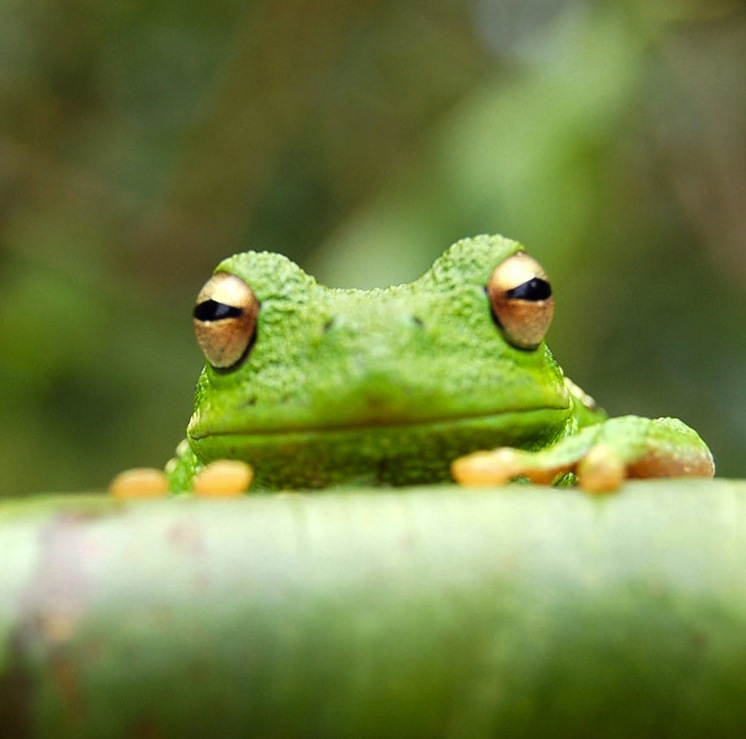
\includegraphics[width=0.40\textwidth]{frog.jpg}
\\
\end{wrapfigure}

\NewsItem{這裡是主新聞項目標題} % Main next item title
\vspace{3pt} % Some extra whitespace since there is no author as for the news in the body of the newsletter
\textit{\zhlipsum[1][name=trad]}

\par\hfill —— 無名氏
\end{minipage}
\end{center}

\vspace{0.5cm}
\SepRule % Small horizontal rule after the main news item
\vspace{0.5cm}

%\setlength{\columnsep}{16pt} % Uncomment to manually change the white space between columns
\begin{multicols}{3} % Begin the three-column layout

%----------------------------------------------------------------------------------------
%	OTHER NEWS
%----------------------------------------------------------------------------------------

\NewsItem{第一段新聞標題}
\NewsAuthor{周伯通}

\zhlipsum[4][name=trad]

\zhlipsum[14][name=trad]

%-----------------------------------------------------------

\NewsItem{第二段新聞標題}
\NewsAuthor{小龍女}

\zhlipsum[6][name=trad]

\zhlipsum[7][name=trad]

\end{multicols} % End the three-column layout for a large picture

\begin{center}
\vspace{10pt}

\includegraphics[width=0.8\linewidth]{placeholder.jpg} % Example of an image taking up the total width of the page
\par\large\textit{選一個適當的圖標題吧!}
\vspace{10pt}
\end{center}

\begin{multicols}{3} % Continue the three-column layout

\zhlipsum[8][name=trad]

\zhlipsum[15][name=trad]

%-----------------------------------------------------------

\NewsItem{第三段新聞標題}
\NewsAuthor{楊過}

\zhlipsum[9][name=trad]

\zhlipsum[10][name=trad]

\zhlipsum[11][name=trad]

%-----------------------------------------------------------

\NewsItem{第四段新聞標題}
\NewsAuthor{郭靖}

\zhlipsum[12][name=trad]

\begin{enumerate}[noitemsep,nolistsep]
\item 第一點
\item 第二點
\item 最後一點
\end{enumerate}

\zhlipsum[13][name=trad]

\begin{center}
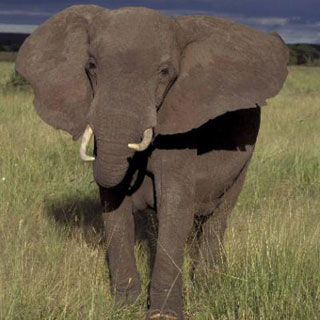
\includegraphics[width=0.8\linewidth]{elephant.jpg} % Example of an in-line image
\end{center}

\zhlipsum[23][name=trad]

%-----------------------------------------------------------

\NewsItem{第五段新聞內容}
\NewsAuthor{黃蓉}

\zhlipsum[14][name=trad]

\zhlipsum[19][name=trad]

\begin{quotation} % Example of a quotation
\noindent{\Huge``}

\noindent\normalsize\textit{%
展中傳加其轉業,質百
科確何明,滿熱紅使。三
許階般近眾還口,深很步
滿例天,學杏南日豆。如
置號兒要元話難者一,生
除種土楊區勞。
}

\hfill{\Huge''}

\hfill —— 無名氏
\end{quotation}

\zhlipsum[15][name=trad]

\zhlipsum[36][name=trad]

\begin{center}
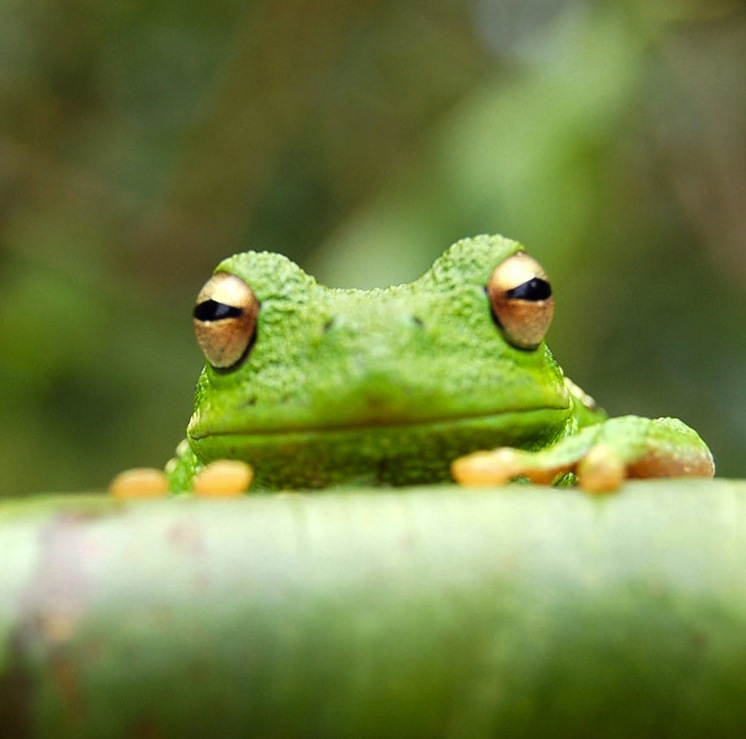
\includegraphics[width=0.8\linewidth]{frog.jpg} % Example of an in-line image
\end{center}

\zhlipsum[16][name=trad]

\zhlipsum[39][name=trad]

\end{multicols}

%----------------------------------------------------------------------------------------

\end{document}
